\section{Blockchain}
Dieses Kapitel konzentriert sich darauf ein tieferes Verständnis für die Funktionsweise einer Blockchain
zu vermitteln. Hierbei werden zunächst der Aufbau und elementare Methoden und Komponenten erläutert.
Des Weiteren wird gezeigt, wie die Technologie bereits im Finanzsektor eingesetzt wird und welches Potenzial
sie in diesem Bereich bietet.


\subsection{Aufbau und Funktionsweise einer Blockchain}
Um das Potential der Blockchain-Technologie zu erkennen, ist es eine Notwendigkeit zunächst ein Verständnis 
für die zugrundeliegenden Prinzipien und den daraus resultierenden Eigenschaften zu erlangen.



%Um die Verwendung von Blockchains im Finanzsektor besser zu verstehen, wird im Folgenden auf den Aufbau und die Komponenten näher eingegangen.


\subsubsection{Hash-Funktion}
Ein elementarer Grundbaustein einer Blockchain ist die Bildung eines Hashes.
\glqq Eine Hash-Funktion bildet eine beliebig gro\ss e Menge an Eingabedaten [...] auf eine Zahl von 
fixer Grö\ss e ab, den sogenannten Hashwert\grqq{} \cite[p.~6]{fill2020blockchain}.
Die Hash-Funktion soll darüber hinaus drei wichtige Eigenschaften besitzen.
Das Diffusionsprinzip beschreibt eine deutliche Änderung des Hashwertes bei einem leicht
abgeänderten Eingabewert. Dadurch können unterschiedliche Eingaben sofort erkannt werden.
Das Konfusionsprinzip beschreibt die Eigenschaft, dass vom Hashwert nicht auf den Eingabewert
geschlossen werden kann. Beim Vergleich zweier Hashwerte von Eingaben mit einer minimalen
Änderung kann nichtmal auf die Position der Abweichung geschlossen werden.
Zuletzt ist die Kollisionsresistenz insbesondere im Bereich der Kryptographie relevant.
% Eine Kollision tritt dann auf, wenn zwei unterschiedliche Eingaben auf denselben Hash abgebildet werden. 
Die Hash-Funktion soll hierfür möglichst vermeiden zwei unterschiedliche Eingabewerte
auf denselben Hashwert abzubilden.
\cite[p.~6ff]{fill2020blockchain} 

\subsubsection{Aufbau einer Blockchain}
Im Block 1 wird zuerst jeweils ein Hash H1 und H2 für die Datenpunkte Transaktion 1 
und Transaktion 2 gebildet (siehe \autoref{fig:BC_Aufbau}). Aus diesen Hashes wird dann ein gemeinsamer Hash H12 gebildet, 
der den Block Header 1 darstellt.
Analog zum Block Header 1 wird Block Header 2 erstellt. Zusätzlich enthält dieser eine
Referenz auf den vorigen Block Header 1 und ist somit der Kopf der Kette. Der Block Header 2
kann weiterführend im Block Haeder 3 eines dritten Blocks referenziert werden. 
Durch diese Datenstruktur kann ein involvierter Rechnerknoten die einzelnen Blöcke rekursiv
zurückverfolgen und Einblick in alle zuvor getätigten Transaktionen haben. Darüber
hinaus befindet sich auf jedem Rechnerknoten eine lokal abgespeicherte Kopie der 
Blockchain.
\cite[p.~17f]{fill2020blockchain}

\begin{figure}[h]
    \begin{center}
        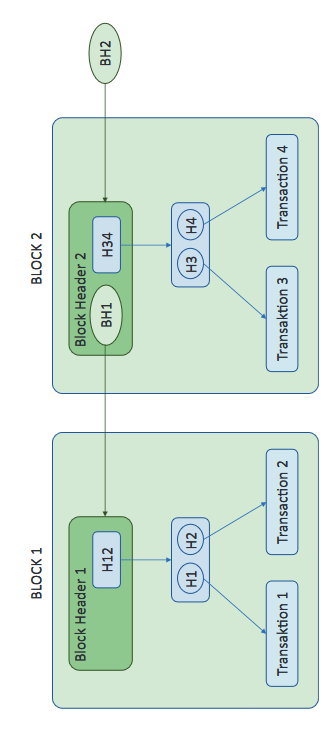
\includegraphics[height=5cm]{BC_Aufbau.png}
    \end{center}
    \quelle{\cite[p.~19]{fill2020blockchain}}
    \captionof{figure}{Aufbau einer Blockchain}
    \label{fig:BC_Aufbau}
\end{figure}

Die Blockchain ist  ein verteiltes Register mit Integritätsgarantie. Die Integrität 
wird hierbei sichergestellt, indem eine Änderung an einem beliebigen Punkt in der
Blockchain eine Anpassung in allen Blöcken nach sich zieht, die eine direkte oder
indirekte Referenz auf diesen Block haben; also im betroffenen Block selbst und den
Nachfolgenden. Änderungen und Erweiterungen der Blockchain werden dank klarer 
und verschlüsselter Eigentumsansprüche, sowie einem Konsensalgorithmus (siehe Kapitel \ref{sec:Erweiterung})
nur dann vorgenommen, wenn sie berechtigt und richtig sind.
% Oder:
% Als Schutzmechanismus werden Änderungen jedoch nur dann vorgenommen, wenn sie durch 
% klare und verschlüsselte Eigentumsansprüche berechtigt sind.
\cite[p.~22]{fill2020blockchain} 

\subsubsection{Erweiterung der Blockchain mit Proof-of-Work}
\label{sec:Erweiterung}
% Erweiterung der Blockchain mittels eines Konsensalgorithmus
Neue Blöcke werden mittels eines Konsensalgorithmus hinzugefügt.
Hierfür muss zuerst ein Rechnerknoten ausgewählt werden, der den neuen Block erstellt. 
Am Beispiel Bitcoin werden die Rechnerknoten auch \glqq Miner\grqq{} genannt.
Um die Dezentralität der Blockchain beizubehalten, kann es keinen Rechnerknoten geben, der einen 
anderen für die Erstellung auswählt. Stattdessen wird die Auswahl per Zufallsprinzip getroffen.
% dezentral --> Verzicht auf Intermediäre
Für die Realisierung der Zufälligkeit gibt es mehrere Ansätze, hier wird auf das
Prinzip \glqq Proof-of-Work\grqq{} eingegangen, welches auch auf der Bitcoin-Plattform angewendet wird.
Es wird ein kryptographisches Puzzle an alle Miner gestellt, das ausschlie\ss lich
durch den erbrachten Rechenaufwand lösbar ist. Daher der Name "Proof-of-Work". 

% Ablauf
Zuerst wird der Block Header um die für das Puzzle nötigen Elemente 
erweitert: Eine Protokollversion für die Erstellung eines neuen Blocks, einen Zeitstempel mit
dem Zeitpunkt des Erstellens, einem Target als Angabe des Schwierigkeitsgrades des Puzzles
und einer Nonce (Number used once) als Beweis der Lösung des Puzzles (siehe \autoref{fig:BC_Erweiterung}).
% nye
Aus diesen zusätzlichen Elemente wird zusammen mit der Referenz BH1 auf den vorangehenden 
Block Header und der Wurzel H34 des Hash-Baumes auf die Transaktionsdaten ein gemeinsamer 
Hashwert errechnet. 
Das Ziel des Puzzles ist einen Hashwert zu generieren, der kleiner als das Target ist. Die 
Schwierigkeit ergibt sich damit indirekt proportional zum Target, denn je kleiner es ist, desto
schwieriger ist die Lösungsfindung und umgekehrt.
Die Miner haben einzig die Nonce als veränderbaren Wert zur Verfügung, um verschiedene Hashes zu generieren. 
Wurde das Rätsel gelöst, wird der neue Block zusammen mit der Nonce an alle anderen Miner zur Prüfung
geschickt.
Zuletzt wird dieser neue Block in die Blockchain aufgenommen, sofern er validiert und 
fehlerfrei ist, ansonsten wird dieser verworfen.
\cite[p.~22ff]{fill2020blockchain}


    
\begin{figure}[h]
    \begin{center}
        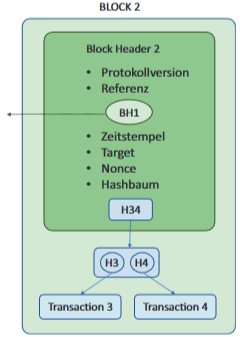
\includegraphics[height=5cm]{BC_Erweiterung.png}
    \end{center}
    \quelle{\cite[p.~24]{fill2020blockchain}}
    \caption{erweiterter Block Header für Proof-of-Work}
    \label{fig:BC_Erweiterung}
\end{figure}



\newpage
\subsection{Einsatzgebiete im Finanzsektor}
Die Blockchain-Technologie ist schon heute in vielen Bereichen des Finanzsektors etabliert und hat viele 
Prozessabläufe optimieren können. In diesem Kapitel werden die grundlegenden Anwendungsgebiete aufgezeigt
und anschlie\ss end auf deren Potential im Finanzsektor eingegangen.



\subsubsection{Transaktionen}
Der Kryptomarkt ist der wohl bekannteste Bereich, welcher auf der Blockchain-Technologie basiert.
%in der die Blockchain ein grundlegender Bestandteil ist. 
Die stärksten Kryptowährungen sind Bitcoin und Ethereum. 
Die Blockchain gewährleistet die Sicherheit und Nachvollziehbarkeit von Transaktionen. 
\cite[p.~168]{chowdhary2025smart}
Die Sicherheit wird durch die Nutzung eines Konsensalgorithmus erreicht, welcher nur validierte 
Änderungen erlaubt. Die Nachvollziehbarkeit wird  durch den Aufbau der Blockchain erreicht, da stets 
alle vorherigen Transaktionen einsehbar sind, indem die Header-Referenzen rekursiv zurückverfolgt
werden können (vgl \autoref{fig:BC_Aufbau}).
% Verweis auf vorher verifizierte Blöcke & vollst. Kopie auf jedem teilnehmenden Gerät.
Im traditionellen Zahlungsverkehr würden Banken und andere Zahlungsdienstleister die 
Vertrauenswürdigkeit der Transaktionsakteure beglaubigen.
Das Zusammenspiel der Datenintegrität, Nachvollziehbarkeit und dezentralen Struktur der
Blockchain ermöglicht den Verzicht auf diese Intermediäre. Stattdessen können digitale 
Währungseinheiten in einem Peer-to-Peer Netzwerk ausgetauscht werden.
\cite[p.~32]{fill2020blockchain}
%\cite[p.~11]{pirafelnerblockchaintechnologie}
Da die Blockchain über Netzwerke agiert, ist die Technologie unbetroffen von Ländergrenzen.
Somit sind die Transaktionsgebühren kostengünstiger, da nur eine Gebühr für 
die Miner anfällt und selten zusätzliche Gebühren für einen Währungswechsel.
\cite[p.~167]{chowdhary2025smart}


\subsubsection{Smart Contracts}
\label{sec:SmartContracts}
Smart Contracts sind digitalisierte und automatisierte Verträge.
\cite[p.~14]{pirafelnerblockchaintechnologie}
Treten die in ihnen definierten Bedingungen ein, so werden die einprogrammierten Aktionen
ausgeführt.
\cite[p.~55f]{fill2020blockchain}
% technische Umsetzung
Voraussetzung ist, dass die Blockchain-Plattform Smart Contracts in Form von 
Befehlssätzen unterstützt. Die Bitcoin-Plattform unterstützt zum Beispiel nur rudimentäre
Skripte mit denen sich hauptsächlich weitere Transaktionen automatisieren lassen. 

Die Ethereum-Plattform hingegen stellt einen viel umfangreicheren Befehlssatz
zur Verfügung. Dieser ist sogar Turing-Vollständig, wodurch er dieselbe Mächtigkeit wie gängige
Programmiersprachen besitzt.
Die bekannteste Programmiersprache für die Umsetzung von Smart Contracts auf der Ethereum-Blockchain 
ist Solidity, die erstmals 2014 von Dr. Gavin Wood vorgestellt wurde. Da die Ausführung eines Smart Contracts
in den einzelnen Rechnerknoten, also bei den Minern, stattfindet, ist es unerlässlich, 
dass die verwendete Sprache auf jeder Rechnerarchitektur interpretiert werden kann.
% Die wichtigste Eigenschaft für jede Programmiersprache um Smart Contracts zu definieren ist, dass sie auf jeder Rechnerarchitektur, unabhängig von der Hard-Ware und dem verwendeten Prozessor, funktioniert. 
Dazu wird der Code des Smart Contract vom Compiler in 
Bytecode umgewandelt und als dieser durch eine Transaktion in die Blockchain 
aufgenommen. % eingefügt
Die Blockchain wird also um einen Block, der den Smart Contract beinhaltet, erweitert.
%Ausführung eines SC
Sobald ein Smart Contract von einer Transaktion aufgerufen wird, wird der Bytecode 
auf der Ethereum Virtual Machine interpretiert.
Ein Smart Contract hat während der Ausführung Zugriff auf verschiedene Daten innerhalb der 
Blockchain. 
% Daten weiter spezifizieren?
% Variation für Inforamtionszugriff:
Darunter zählen alle spezifizierten Daten im Smart Contract selbst, wie eigene Variablen
und Datenstrukturen. Informationen der aufrufenden Transaktion sind ebenfalls zugänglich, um 
mittels der mitgelieferten Adresse die Identität des Aufrufers
zu authentifizieren. Aus der gesamten Blockchain kann ein Smart Contract neben
allgemein zugänglichen Informationen auch auf bestimmte Daten zugreifen, wie z.B. 
Tokens die dem Aufrufer zugeschrieben sind (vgl Kapitel \ref{sec:Tokenization}).
Sind zur Ausführung des Contracts externe Informationen relevant, ist die Einbindung von Oracles
eine gängige Praxis. Mithilfe dieser kann auf Datenbanken oder andere Datenspeicher zugegriffen werden.
Ein Smart Contract kann auch weitere Smart Contracts in der Blockchain aufrufen und so 
mehrere Automationen in Reihe schalten oder Informationen für alle Rechnerknoten in Events
einsehbar gestalten.
\cite[p.~57ff]{fill2020blockchain}

% Anwendungsgebiete und Vorteile spezifizieren
Die Eigenschaft finanzielle Vertragsbestimmungen automatisch abzuhandeln macht Smart Contracts 
besonders für standardisierte Verträge effizient. Sobald die im Smart Contract definierten Bedingungen
eintreten, wird automatisch eine Transaktion ausgeführt und der Vertrag damit erfüllt.
So können manuelle Prozessschritte reduziert werden, wodurch einhergehende Fehlerquellen
der menschlichen Bearbeitung reduziert werden können. 
Ein konkreter Anwendungsfall in Versicherungsfirmen ist ein Versicherungsanspruch.
\cite[p.~168f]{chowdhary2025smart}
Dabei ist vor allem die Höhe des Anspruches sowohl für das Unternehmen, als auch für den
Anspruchsteller relevant, jedoch ist diese oft von vielen Faktoren abhängig. Um die genaue Höhe zu bestimmen,
können die relevanten Parameter z.B. in einem externen Tool aufgenommen werden, auf die der Smart Contract
über Oracles zugreifen kann. Die Gesamthöhe wird dann innerhalb des Contracts errechnet und kann automatisch
an den Anspruchsteller in Form einer Transaktion überwiesen werden. 
Für Versicherungsfirmen bietet die Integration einer Blockchain-Technologie zusammen mit Smart Contracts
auch einen Schutz vor Versicherungsbetrug. Die Transparenz aller getätigter Transaktionen
und geleisteter Services können auf der Blockchain gespeichert werden und sind damit für einen Smart Contract
einsehbar. Zudem sind die Daten durch das Konsensverfahren der Blockchain sicher vor 
Manipulationen. 
Dadurch können falsche Forderungen sofort erkannt und die weitere Ausführung des Smart
Contracts abgebrochen werden.
\cite[p.~10]{chenthara2021privacy}

Andere Einsatzmöglichkeiten sind im Bankwesen eine Darlehensvergabe oder das Trading
mit Derivaten. \cite[p.~168f]{chowdhary2025smart}
Für Darlehensvergaben müsste man sich weiterhin persönlich auf die Vertragsbedingungen 
einigen. Danach können diese im Smart Contract aufgenommen werden und das Darlehen wird 
 nach Erfüllung der Bedingungen automatisch ausgezahlt, was Warte- und Bearbeitungszeiten verkürzt.
\cite{Gronemann2018darlehen}
% Risiken
Bei der Nutzung von Smart Contracts ist es eine Notwendigkeit, dass diese von Beginn an genau 
definiert sind und alle Randfälle beachtet wurden, da sie nach der Aufnahme in die Blockchain 
nicht mehr angepasst werden können. 
\cite[p.~58]{fill2020blockchain}

% Anfechtbarkeit (pfilner, p.14)
% Anfechtbarkeit bei Verträgen über mehrere Länder

% Nachteile
% Aber aufpassen dass Ausführungsgebühr ausreicht, sonst Ausführung gecancelt und Betrag nicht zurückerstattet
% Funktion zum deaktivieren des Vertrags nur Optional. Wenn nicht vorhanden, ist der Smart Contract also immer aktiviert.



\subsubsection{Tokenization von Assets}
\label{sec:Tokenization}
Der Prozess \glqq Tokenization\grqq{} beschreibt die Darstellung von finanziellen oder physischen
Wertgegenständen als Blockchain-basierte Tokens. Die Erstellung der Tokens geschieht durch 
eine bestimmte Art von Initial Coin Offering (ICO), die den Wert des Gegenstands in Security Tokens 
darstellt.
\cite[p.~82]{gupta2020tokenization}
Die Abgrenzung zu anderen ICOs besteht darin, dass die Anzahl der Tokens von Beginn an begrenzt ist.
Bei ICOs im Allgemeinen ist das nur optional.
\cite[p.66]{fill2020blockchain}
Es ergeben sich hauptsächlich einige Vorteile sowohl liquide, als auch nicht-liquide Assets in Tokens zu 
repräsentieren.

Ein Vorteil ist, dass die Liquidität erhöht wird.
Vor allem nicht-liquide Assets profitieren stark davon, dass die Tokens unkompliziert in digitalen
Wallets gespeichert werden können. Dadurch wird der Handel mit ebendiesen ungemein erleichtert, wodurch
sich ein grö\ss erer Investoren- und Interessentenkreis eröffnet.
Zudem finden die Vorteile von Transaktionen mit Blockchain-basierten Währungen hier ebenfalls Anwendung.
Die Transaktionen werden schneller und günstiger ausgeführt, da hier auf Smart Contracts zur 
Automatisierung zurückgegriffen werden kann. 
Des Weiteren bietet ein Token eine höhere Transparenz als Transaktionen auf einer Blockchain.
Im Token wird eine vollständige und unveränderliche Historie der Besitzer, auch Token-Holder gennant,
gespeichert. Zusätzlich sind die Rechte und Verpflichtungen, die mit dem Token einhergehen, darauf 
vermerkt.
Diese Informationen definieren eindeutig die Ansprüche der Akteure und vermeiden eine Anonymität in
der Transaktion.
Zuletzt wird die Zugänglichkeit, die Accessibility, zu jeder Art von Asset verbessert. 
Der Mindestbetrag für Assets kann durch Tokens gesenkt werden, da diese leicht teilbar sind und so 
kleinste Bruchteile des Assets gehandelt werden können.
\cite[p.~82]{gupta2020tokenization}

Tokens vereinen demnach eine hohe Liquidität und Zugänglichkeit durch geringe Mindestbetrage.
Diese Kombination öffnet den Markt für viele Privatanleger und Kleinstinvestoren und schafft dadurch
eine finanzielle Inklusion für diese Personengruppen.
\cite[p.~167]{chowdhary2025smart}


% Erleichtert es privaten Anlegern
% Erleichtert es kleinen / mittelständischen Unternehmen auf der Börse, da eine breitere
% Masse investieren kann. -> Bekäme ich einen Dollar von 1 Mio. Menschen, dann hätte ich 1 Mio. Dollar.



% \subsubsection{Smart Grid im Energiesektor}
% Besser im Kapitel Nachhaltigkeit!
% \cite[p.~72]{fill2020blockchain}


% \subsection{Ausblick und Risiken bei der Integration von Blockchains}



% Besser im Fazit: Quantum Computing:
% extrem effizient darin eine Primfaktorzerlegung durchzuführen.

% Daten werden gesammelt, selbst wenn sie nicht direkt von Menschen abgerufen werden (Versicherungen).
% Dennoch sind diese Daten höchst sensibel und ein Datenleck kann nie sicher ausgeschlossen werden, da 
% es kein sicheres System gibt. Nur Systeme, deren Lücken noch nicht gefunden wurden.
